\section{CPU Parallel Framework Overview}

\subsection{Framework Comparison}
\begin{frame}[fragile]{\emoji{balance-scale} Parallel Programming Framework Comparison}
	\begin{table}[h]
		\centering
		\small
		\begin{tabular}{|l|c|c|c|}
			\hline
			\textbf{Feature}     & \textbf{OpenMP}    & \textbf{MPI}         & \textbf{C++ Thread} \\
			\hline
			Programming Model    & Compiler Directive & Message Passing      & Native API          \\
			Memory Model         & Shared Memory      & Distributed Memory   & Shared Memory       \\
			Learning Curve       & Easy               & Moderate             & Moderate            \\
			Control Granularity  & Coarse             & Fine                 & Very Fine           \\
			Debugging Difficulty & Low                & High                 & High                \\
			\hline
			\textbf{Use Cases}   & Regular Loops      & Cross-node Computing & Complex Task Sched. \\
			                     & Data Parallelism   & Large-scale HPC      & Event-driven Apps   \\
			\hline
		\end{tabular}
	\end{table}

	\vspace{1em}
	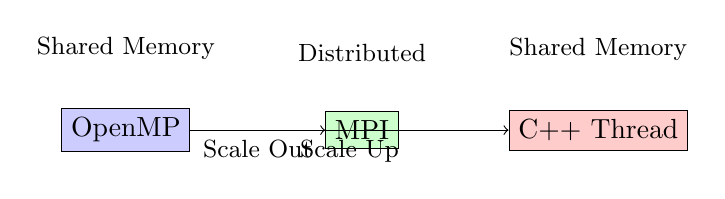
\begin{tikzpicture}
		\node[draw, rectangle, fill=blue!20] (openmp) at (0,0) {OpenMP};
		\node[draw, rectangle, fill=green!20] (mpi) at (3,0) {MPI};
		\node[draw, rectangle, fill=red!20] (cpp) at (6,0) {C++ Thread};

		\node[above] at ([yshift=0.5cm]openmp.north) {\small Shared Memory};
		\node[above] at ([yshift=0.5cm]mpi.north) {\small Distributed};
		\node[above] at ([yshift=0.5cm]cpp.north) {\small Shared Memory};

		\draw[->] (openmp) -- node[midway, below] {\small Scale Up} (cpp);
		\draw[->] (openmp) -- node[midway, below] {\small Scale Out} (mpi);
	\end{tikzpicture}
\end{frame}

\begin{frame}[fragile]{\emoji{gear} When to Use Which Framework?}
	\begin{tikzpicture}[node distance=2cm]
		\node[draw, rectangle, fill=yellow!20] (start) {Parallel Task};

		\node[draw, diamond, fill=blue!10] (memory) at ([yshift=-2cm]start.south) {Data Distribution?};

		\node[draw, rectangle, fill=green!20] (openmp) at ([shift={(-2cm,-2cm)}]memory.south west) {OpenMP};
		\node[draw, rectangle, fill=red!20] (distributed) at ([shift={(2cm,-2cm)}]memory.south east) {Cross-node?};

		\node[draw, rectangle, fill=orange!20] (cpp) at ([shift={(-2cm,-2cm)}]distributed.south west) {C++ Thread};
		\node[draw, rectangle, fill=purple!20] (mpi) at ([shift={(2cm,-2cm)}]distributed.south east) {MPI};

		\draw[->] (start) -- (memory);
		\draw[->] (memory) -- node[left] {Regular Loop} (openmp);
		\draw[->] (memory) -- node[right] {Complex Logic} (distributed);
		\draw[->] (distributed) -- node[left] {Single Node} (cpp);
		\draw[->] (distributed) -- node[right] {Multi-node} (mpi);
	\end{tikzpicture}

	\vspace{1em}
	\textbf{Decision Factors:}
	\begin{itemize}
		\item \textbf{Data locality}: Shared vs distributed memory
		\item \textbf{Task complexity}: Regular patterns vs irregular workloads
		\item \textbf{Scale requirements}: Single node vs cluster
		\item \textbf{Control needs}: Coarse-grained vs fine-grained control
	\end{itemize}
\end{frame}

\subsection{Thread Lifecycle Management}
\begin{frame}[fragile]{\emoji{thread} C++ Thread Basics: Creation and Management}
	\begin{columns}
		\begin{column}{0.5\textwidth}
			\textbf{C pthread Example}
			\begin{minted}{c}
#include <pthread.h>
#include <stdio.h>

void* worker(void* arg) {
    int id = *(int*)arg;
    printf("Worker %d running\n", id);
    return NULL;
}

int main() {
    pthread_t threads[4];
    int ids[4];

    for(int i = 0; i < 4; i++) {
        ids[i] = i;
        pthread_create(&threads[i], NULL,
                       worker, &ids[i]);
    }

    for(int i = 0; i < 4; i++) {
        pthread_join(threads[i], NULL);
    }

    return 0;
}
			\end{minted}
		\end{column}
		\begin{column}{0.5\textwidth}
			\textbf{C++ std::thread Example}
			\begin{minted}{cpp}
#include <thread>
#include <vector>
#include <iostream>

void worker(int id) {
    std::cout << "Worker " << id
              << " running" << std::endl;
}

int main() {
    std::vector<std::thread> threads;

    // Create threads
    for(int i = 0; i < 4; i++) {
        threads.emplace_back(worker, i);
    }

    // Wait for completion
    for(auto& t : threads) {
        t.join();
    }

    return 0;
}
			\end{minted}
		\end{column}
	\end{columns}

	\vspace{0.5em}
	\textbf{C++ Advantages:}
	\begin{itemize}
		\item Type-safe parameter passing
		\item RAII automatic resource management
		\item Exception safety
	\end{itemize}
\end{frame}

\begin{frame}[fragile]{\emoji{warning} Parameter Passing Pitfalls}
	\begin{minted}{cpp}
#include <thread>
#include <iostream>
#include <vector>

void print_value(int val) {
    std::cout << "Value: " << val << std::endl;
}

void increment(int& val) {
    val++;
}

int main() {
    int x = 42;

    // Pass by value - safe
    std::thread t1(print_value, x);

    // This won't compile - can't pass reference directly
    // std::thread t2(increment, x);

    // Correct way to pass reference
    std::thread t2(increment, std::ref(x));

    // Dangerous - reference to local variable
    std::vector<std::thread> threads;
    for(int i = 0; i < 3; i++) {
        // threads.emplace_back(print_value, i);  // Dangerous!
        threads.emplace_back(print_value, i);     // OK - copy
    }

    t1.join();
    t2.join();

    for(auto& t : threads) {
        t.join();
    }

    std::cout << "Final x: " << x << std::endl;
    return 0;
}
	\end{minted}
\end{frame}

\begin{frame}[fragile]{\emoji{laptop} Hands-on: Multi-threaded Array Sum}
	\textbf{Task}: Calculate sum of array using multiple threads

	\begin{minted}{cpp}
#include <thread>
#include <vector>
#include <numeric>
#include <iostream>

void partial_sum(const std::vector<int>& arr,
                 size_t start, size_t end,
                 long long& result) {
    result = 0;
    for(size_t i = start; i < end; i++) {
        result += arr[i];
    }
}

int main() {
    const size_t SIZE = 1000000;
    std::vector<int> data(SIZE, 1);  // All elements = 1

    const int NUM_THREADS = 4;
    std::vector<std::thread> threads;
    std::vector<long long> partial_results(NUM_THREADS, 0);

    size_t chunk_size = SIZE / NUM_THREADS;

    // Create worker threads
    for(int i = 0; i < NUM_THREADS; i++) {
        size_t start = i * chunk_size;
        size_t end = (i == NUM_THREADS-1) ? SIZE : (i+1) * chunk_size;

        threads.emplace_back(partial_sum, std::cref(data),
                           start, end, std::ref(partial_results[i]));
    }

    // Wait for completion and sum results
    for(auto& t : threads) {
        t.join();
    }

    long long total = std::accumulate(partial_results.begin(),
                                    partial_results.end(), 0LL);

    std::cout << "Total sum: " << total << std::endl;
    return 0;
}
	\end{minted}
\end{frame}
